\documentclass[12pt, aspectratio=141]{beamer}

\definecolor{jrouge}{HTML}{CB3C33}
\definecolor{jvert}{HTML}{389826}
\definecolor{jbleu}{HTML}{4063D8}
\definecolor{jviolet}{HTML}{9558B2}
\definecolor{lightred}{HTML}{fcf3f3}
\definecolor{lightgreen}{HTML}{e1f6db}
\definecolor{lightpurple}{HTML}{f4eef7}
\definecolor{lightgrey}{gray}{0.95}

\mode<presentation>
{
	\usetheme{default}
	\usecolortheme{rose}
	%	\useoutertheme{smoothbars}
	\useinnertheme{circles}
	
	\definecolor{beamer@blendedblue}{HTML}{4063D8}
	%\definecolor{titlemustard}{rgb}{0.6,0.6,0.0}
	%\setbeamercolor{title}{bg=titlemustard}
	\setbeamercolor{normal text}{fg=black}
	\setbeamercolor{alerted text}{fg=jrouge}
	\setbeamerfont{title}{shape=\bfseries}
	\setbeamercolor{example text}{fg=jvert}
	
	%\setbeamercolor{structure}{fg=beamer@blendedblue}
	\setbeamertemplate{navigation symbols}{}
	\setbeamertemplate{footline}{\color{black!50}\hfill\scriptsize\insertpagenumber\hspace{2em}\vspace{2em}}
}

\usepackage{natbib}
%\renewcommand{\citenumfont}[1]{{\tiny#1}}
\renewcommand{\citenumfont}[1]{}
\bibpunct{}{};s;;

\usepackage[french]{babel}
\usepackage[mathletters]{ucs}
\usepackage[utf8x]{inputenc}
\usepackage[T1]{fontenc}
% Or whatever. Note that the encoding and the font should match. If T1
% does not look nice, try deleting the line with the fontenc.
% Alternative for XeLaTeX:
%\usefonttheme{professionalfonts}
%\usepackage{fontspec}
%\setmonofont{JuliaMono}
%\setdefaultlanguage{french}
%\usepackage{unicode-math}

\usepackage{subcaption}

\usepackage{array}
\usepackage{multirow}
\usepackage{setspace}
\usepackage{soul}
\usepackage{amssymb}
\usepackage{mathrsfs}
\usepackage{bbm}
\usepackage{svg}

\usepackage{tikz}
\usetikzlibrary{scopes, backgrounds, arrows, automata, positioning, patterns, calc, decorations.pathmorphing, decorations.pathreplacing, arrows.meta}

\usepackage{hyperref}
\usepackage{ragged2e}
\usepackage{graphicx}
\usepackage{amsmath}
\usepackage{aeguill}

\usepackage{algorithm}
\usepackage{algpseudocode}
\usepackage{stmaryrd}
\usepackage{moresize}

\newcommand{\llbra}{\left\llbracket}
\newcommand{\rrbra}{\right\rrbracket}
\renewcommand{\brack}[1]{\ensuremath{\llbra#1\rrbra}}
\newcommand{\der}[2]{#1^{\ensuremath{\left(#2\right)}}}
\newcommand{\paren}[1]{\ensuremath{\left(#1\right)}}
\newcommand{\abs}[1]{\ensuremath{\left|#1\right|}}
\newcommand{\norm}[1]{\ensuremath{\left\|#1\right\|}}
\newcommand{\interval}[1]{\ensuremath{\left[#1\right]}}
\newcommand{\set}[2]{\ensuremath{\left\{#1\,\middle|\,#2\right\}}}
\newcommand{\R}{\ensuremath{\mathcal R}}
\newcommand{\N}{\ensuremath{\mathcal N}}
\newcommand{\cont}[1]{\mathcal{C}^{#1}}
\newcommand{\tends}[2]{\underset{#1\to #2}{\longrightarrow}}
\newcommand{\seq}[3]{\ensuremath{\left(#1_{#2}\right)_{#2\in#3}}}
\newcommand{\matr}[2]{\mathcal{M}_{#1}\paren{#2}}
\newcommand{\matrRect}[3]{\mathcal{M}_{#1,#2}\paren{#3}}
\newcommand{\Id}{\text{Id}}
\newenvironment{disj}[1]{\left\{\begin{array}{#1}} {\end{array}\right.}

\usepackage{siunitx}


\newenvironment{changemargin}[2]{%
	\begin{list}{}{%
			%\setlength{\topsep}{0pt}%
			\setlength{\leftmargin}{#1}%
			\setlength{\rightmargin}{#2}%
			\setlength{\listparindent}{\parindent}%
			\setlength{\itemindent}{\parindent}%
			\setlength{\parsep}{\parskip}%
		}%
		\item[]}{\end{list}}

\defbeamertemplate{section page}{mruffel}[1][]{%
	\begin{centering}
		{\usebeamerfont{section name}\usebeamercolor[fg]{section name}#1
			\vskip1em\par
			
			\begin{beamercolorbox}[sep=12pt,center,rounded=true,shadow=true]{part title}
				\usebeamerfont{section title}\insertsection\par
		\end{beamercolorbox}}
	\end{centering}
}



% If you have a file called "university-logo-filename.xxx", where xxx
% is a graphic format that can be processed by latex or pdflatex,
% resp., then you can add a logo as follows:

\pgfdeclareimage[height=0.5cm]{Mines}{../figures/Mines.pdf}
\logo{\begin{tikzpicture}[overlay,remember picture]
		\node[left=0.2cm] at (current page.31){
			\pgfuseimage{Mines}
		};
\end{tikzpicture}}



% Delete this, if you do not want the table of contents to pop up at
% the beginning of each subsection:
%\AtBeginSubsection[]
%{
	%  \begin{frame}<beamer>
		%    \tableofcontents[currentsection,currentsubsection]
		%  \end{frame}
	%}

\AtBeginSection[]
{
	\begin{frame}
		\sectionpage
	\end{frame}
}

% If you wish to uncover everything in a step-wise fashion, uncomment
% the following command: 

%\beamerdefaultoverlayspecification{<+->}

\usepackage{minted}
\usemintedstyle{paraiso-light}
\setminted[julia]{mathescape,linenos,obeytabs,tabsize=4,numbersep=3pt,fontsize=\small,framesep=2mm,autogobble,bgcolor=lightred,escapeinside=££}
\setminted[bash]{mathescape,obeytabs,tabsize=4,numbersep=3pt,fontsize=\small,framesep=2mm,autogobble,bgcolor=lightgrey,escapeinside=££}

\usepackage{lmodern}
%\newcommand{\jl}[1]{\colorbox{lightred}{\small\ttfamily #1}}
\newmintinline[jl]{julia}{}
\newmintinline[jlscript]{julia}{fontsize=\scriptsize}
\newmint[JL]{julia}{}
\newmint[JLa]{julia}{linenos=false}
\newminted{julia}{}
\newenvironment{julia}{\vspace{-0.6em}\VerbatimEnvironment\begin{juliacode}}{\end{juliacode}}
\newminted[jlrepl]{julia}{linenos=false}
\newenvironment{repl}{\vspace{-0.6em}\VerbatimEnvironment\begin{jlrepl}}{\end{jlrepl}}
\newcommand{\q}{\textquotesingle}
\newcommand{\qq}{\textquotedbl}
\newcommand{\jlREPL}{\textcolor{jvert}{\bfseries julia>}}

\DeclareTextFontCommand{\emph}{\color{jrouge}\bfseries}

\newenvironment<>{definition}[1]{%
	\setbeamercolor{block title}{bg=lightgreen}%
	\begin{block}{Définition}{#1}}{\end{block}}

\newenvironment<>{convention}[1]{%
	\setbeamercolor{block title}{bg=lightpurple}%
	\begin{block}{Convention}{#1}}{\end{block}}

\usepackage{xspace}
\newcommand{\expr}{\ensuremath{\left\langle\textit{expr}\right\rangle}\xspace}
\newcommand{\expra}[1]{\ensuremath{\left\langle\textit{expr}_{#1}\right\rangle}\xspace}
\newcommand{\bexpr}{\ensuremath{\left\langle\textit{bexpr}\right\rangle}\xspace}
\newcommand{\bexpra}[1]{\ensuremath{\left\langle\textit{bexpr}_{#1}\right\rangle}\xspace}
\newcommand{\type}{\ensuremath{\left\langle\textit{type}\right\rangle}\xspace}
\newcommand{\typea}[1]{\ensuremath{\left\langle\textit{type}_{#1}\right\rangle}\xspace}


\title{Apprentissage de la programmation en Julia}

\subtitle{Interpolation, optimisation}

\author{Lionel~Zoubritzky\inst{}}

\institute{Mines Paris -- PSL}

\date{12/2024}

\begin{document}
\setbeamertemplate{section page}[mruffel]

\begin{frame}
	\titlepage
\end{frame}

\begin{frame}{Interpolation et extrapolation}
	\begin{definition}{}
		\emph{Interpoler} une fonction $f$ en des \emph{n\oe uds} $x_1, x_2, \ldots, x_n$ consiste à trouver une fonction $g$ telle que $\forall i\in\brack{1,n},\ g(x_i) = f(x_i)$.
		
		La qualité d'une interpolation est déterminée par :
		\begin{itemize}
			\item La proximité de $f$ et $g$ sur l'enveloppe convexe des $\seq xi{\brack{1,n}}$ ;
			\item La simplicité et la régularité de $g$.
		\end{itemize}
	\end{definition}

	\begin{definition}{}
		\emph{Extrapoler} une fonction $f$ définie sur $\Omega$ \emph{en dehors d'un espace $I\subset\Omega$} consiste à trouver $g$ définie sur $\Omega$ telle que $\forall x\in I,\ g(x) = f(x)$.

		La qualité d'une extrapolation est déterminée par :
		\begin{itemize}
			\item La proximité de $f$ et $g$ sur $\Omega$ ;
			\item La simplicité et la régularité de $g$.
		\end{itemize}
	\end{definition}
\end{frame}

\begin{frame}{Interpolation linéaire}
	La stratégie d'interpolation la plus simple est l'\emph{interpolation linéaire}. Cela consiste à prendre pour $g$ une fonction affine par morceaux, définie par la contrainte $g(x_i) = f(x_i)$.
	\vfill
	
	En 1D : pour $x_i < x < x_{i+1}$, on a :
	\[g(x) = \frac{(x-x_i)\times f(x_{i+1}) + (x_{i+1}-x)\times f(x_i)}{x_{i+1} - x_i}\]
	\vfill

	En dimension supérieure, l'interpolation est généralement réalisée sur une \emph{grille régulière}, c'est-à-dire un ensemble de nœuds $x_{i_1, \ldots, i_N}$ de la forme
	\[x_{i_1,\ldots, i_N} = (\lambda_1 i_1 + \mu_1, \ldots, \lambda_N i_N + \mu_N)\]
	avec chacun des $i_k$ pris sur des intervalles d'entiers.
	\vfill
	
	L'interpolation linéaire permet aussi d'extrapoler de façon affine en dehors de l'enveloppe convexe de $x_i$.
\end{frame}

\begin{frame}{Interpolation de Lagrange}
	L'\emph{interpolateur de Lagrange} d'une fonction $f$ aux nœuds $x_1, \ldots, x_{n+1}$ (distincts) est le polynôme $L$ de degré minimal (au plus $n$) tel que $\forall i\in\brack{1,n+1},\ L(x_i) = f(x_i)$.
	
	Il est donné par la formule :
	\[L(X) = \sum_{i=1}^{n+1} f(x_i)\paren{\prod_{j=1\atop j\neq i}^{n+1} \frac{X - x_j}{x_i - x_j}}\]

	Par rapport à l'interpolation linéaire, l'interpolation de Lagrange présente le grand avantage d'être $\cont{\infty}$.
	En contrepartie :
	\begin{itemize}
		\item Plus le degré $n$ est élevé, plus le temps d'évaluation de $L$ est grand : l'interpolateur n'est pas simple.
		\item Dans certains cas, plus le nombre de $x_i$ est élevé, plus l'écart maximal entre la fonction $f$ et l'interpolateur $P$ augmente (phénomène de Runge).
		\item L'extrapolation est généralement très mauvaise.
	\end{itemize}
\end{frame}

\begin{frame}{Splines}
	Les inconvénients de l'interpolation de Lagrange proviennent de l'augmentation du degré du polynôme. Une solution consiste à utiliser une \emph{spline}, c'est-à-dire une fonction polynomiale par morceaux.
	\vfill

	En 1D, on utilise généralement les \emph{splines cubiques d'Hermite}, pour effectuer une interpolation $\cont1$ d'une fonction $f$ qui vérifie non seulement $g(x_i) = f(x_i)$ aux nœuds $x_i$, mais aussi $g'(x_i) = f'(x_i)$.
	\vfill

	\begin{minipage}{0.6\linewidth}
		Pour une fonction 1D, on définit par morceau $g$ sur $\interval{x_i,x_{i+1}}$ par
		\[\begin{split}
			g(x_i + t(x_{i+1}-x_i)) &= h_{00}(t)\times f(x_i)
			\\&+ h_{01}(t)\times f(x_{i+1})
			\\&+ h_{10}(t)\times \lambda f'(x_{i})
			\\&+ h_{11}(t)\times \lambda f'(x_{i+1})
		\end{split}\]
	\end{minipage}\hfill%
	\begin{minipage}{0.4\linewidth}
		\centering
		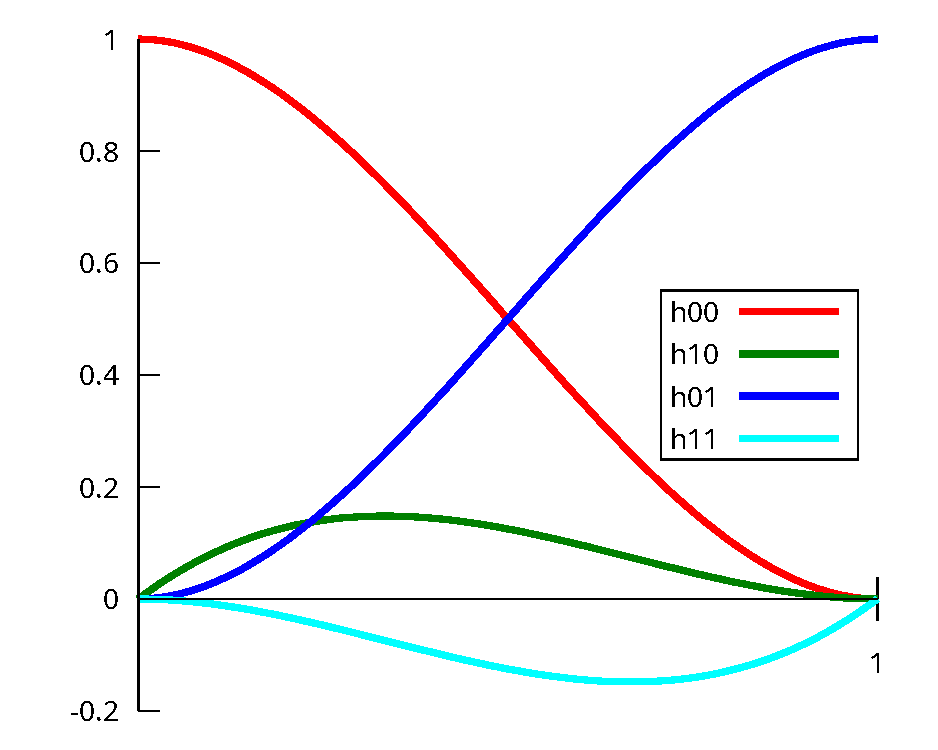
\includegraphics[width=0.9\linewidth]{../figures/HermiteBasis.pdf}
		\vspace{1em}
	\end{minipage}
	avec $\lambda = x_{i+1} - x_i$ et les $h_{ij}$ les polynômes de degré 3 représentés à droite.
\end{frame}

\begin{frame}[fragile]{Usage simple de Interpolations.jl}
	Il existe plusieurs bibliothèques permettant de réaliser des interpolations en Julia. Ce cours présente Interpolations.jl (mais vous pouvez aussi regarder BasicInterpolators.jl, et plus généralement la liste présente sur : {\footnotesize\url{https://juliamath.github.io/Interpolations.jl/latest/other_packages/}}).
	\vfill

	Cette bibliothèque est optimisée pour des interpolations et extrapolations à partir de grilles régulières. Exemple :
	\begin{julia}
		using Statistics: var
		using Interpolations
		# some function that takes a lot of time to run:
		f(x) = var(log(1 + 4x^2/i) + 9sin(x)/sqrt(i) for i in 1:10000)
		xs = 1.0:0.8:20.0  # grid
		itp = cubic_spline_interpolation(xs, f.(xs))  # interpolation
		itp(π)  # interpolated computation
	\end{julia}

	On peut alternativement utiliser \jl{constant_interpolation} (constante par morceaux) ou \jl{linear_interpolation} (interpolation linéaire).
\end{frame}

\begin{frame}{Usage simple de Interpolations.jl}
	\centering
	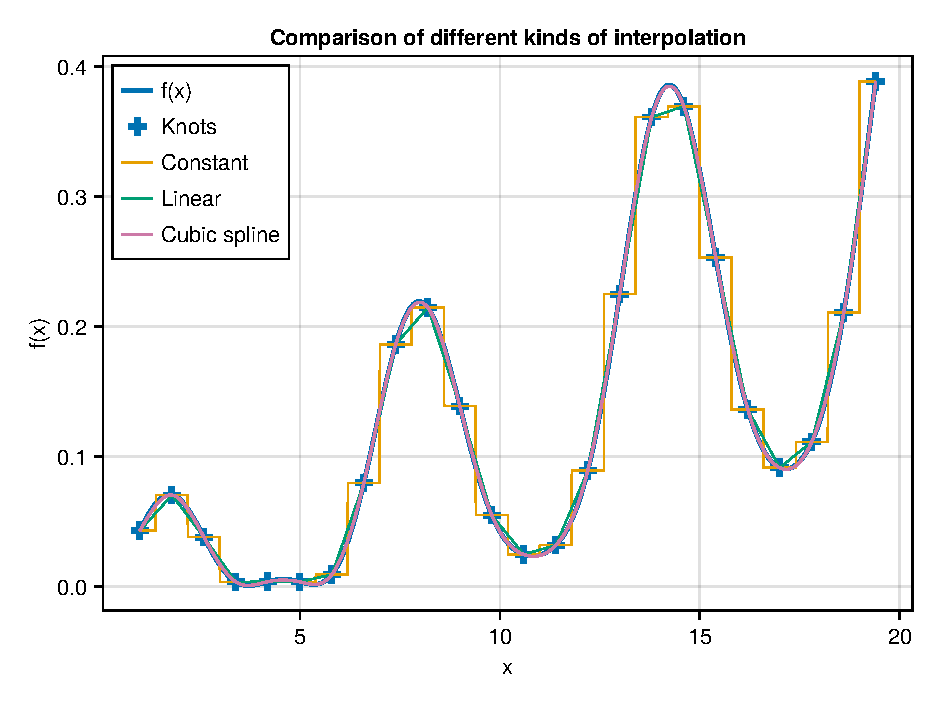
\includegraphics[width=0.9\linewidth]{../figures/interpolation_example.pdf}
\end{frame}

\begin{frame}{Usage détaillé de Interpolations.jl}
	Les trois fonctions comme \jl{cubic_spline_interpolation(xs, A)} sont de simples raccourcis pour trois opérations :

	\begin{itemize}
		\item \jl{itp1 = interpolate(A, alg)} crée un interpolateur sur les valeurs de \jl{A}, ayant pour indices \jl{CartesianIndices(A)}. \jl{alg} peut être \jl{BSpline(...)}, \jl{NoInterp()}, ou un tuple de tels algorithmes.
		
		Exemple : si \jl{A} est une \jl{Matrix} de taille $n\times m$, alors \jl{interpolate(A, (NoInterp(), BSpline(Constant()))} renvoie un interpolateur constant par morceaux de $\brack{1,n}\times\interval{1, m}$ sur \jl{A}.
		\vspace{1em}
		
		\item \jl{itp2 = scale(itp1, xs)} transforme les indices de l'interpolateur pour les faire coïncider avec \jl{xs}. Plusieurs dimensions correspondent à plusieurs arguments \jl{xs}
		
		Exemple : si \jl{A == [f(i, y) for i in 1:4, y in 0.0:0.01:4.0]} et \jl{itp1 = interpolate(A, ...)}, on obtient un interpolateur de \jl{f} avec \jl{scale(itp1, 1:4, 0.0:0.01:4.0)}.
		\vspace{1em}
		
		\item \jl{itp3 = extrapolate(itp, mode)} ajoute la capacité d'extrapolation.
	\end{itemize}
\end{frame}

\begin{frame}{Usage détaillé de Interpolations.jl}
	L'argument de \jl{BSpline(...)} est le type d'interpolation :
	\begin{itemize}
		\item \jl{Constant()} : constant par morceaux. \jl{Constant(Previous)} et \jl{Constant(Next)} déplacent la position de la marche d'escalier.
		\item \jl{Linear()}/\jl{Quadratic(...)}/\jl{Cubic(...)} :  degré 1, 2 ou 3.
	\end{itemize}
	\vspace{0.8em}

	Pour \jl{Quadratic} et \jl{Cubic} qui nécessite des dérivées, on peut spécifier les conditions au bord de la grille, parmi :
	\begin{itemize}
		\item \jl{Flat(...)} : la fonction est constante hors de la grille.
		\item \jl{Line(...)} : la fonction est affine hors de la grille (valeur par défaut).
		\item \jl{Free(...)}\footnote[frame]{Ne peut pas être utilisé pour extrapoler} : garantit un interpolant $\cont3$.
		\item \jl{Periodic(...)} : la fonction est périodique.
		\item \jl{Reflect(...)} : la fonction est réfléchie au bord.
	\end{itemize}
	\vspace{0.5em}
	Chacune de ces conditions prend de plus un argument, qui peut être :
	\begin{itemize}
		\item \jl{OnGrid()} : le bord est le dernier point de la grille (valeur par défaut).
		\item \jl{OnCell()} : le bord est au demi-point fictif après le dernier point.
	\end{itemize}
	\vspace{0.5em}

	Ces conditions au bord servent aussi de \jl{mode} pour extrapoler.\vspace{0.5em}
\end{frame}

\begin{frame}{Ajustement de courbes}
	Les méthodes d'interpolation permettent de trouver des fonctions qui passent \textbf{exactement} par des nœuds donnés, possiblement avec des dérivées données aussi.
	\vfill

	Une interpolation de $n$ points nécessite en général au moins $n$ paramètres. Il est parfois utile d'avoir accès à des modèles encore plus simples.
	\begin{definition}{}
		Étant donné un \emph{modèle} ou courbe paramétrique $g$ qui dépend de paramètres $p_1, p_2, \ldots, p_m$, le problème de l'\emph{ajustement du modèle} ou de la courbe (\textit{curve fitting}) $g$ par rapport à la fonction $f$ aux points $x_1, \ldots x_n$ avec la distance $d$ consiste à trouver les valeurs des paramètres $p_1, p_2, \ldots, p_m$ qui minimisent $d(f(x_i)_{i\in\brack{1,n}}, g_{p_1,\ldots,p_m}(x_i)_{i\in\brack{1,n}})$.
	\end{definition}
	\vfill

	Avec $d$ la distance euclidienne (induite par la norme $\ell^2$), on parle de \emph{méthode des moindres carrés} car cela consiste à minimiser : \vspace{-0.5em}
	\[\sum_{i=1}^n\norm{f(x_i) - \text{g}_{p_1,p_2,\ldots,p_m}(x_i)}^2\]
	\vspace{-2em}
\end{frame}

\begin{frame}{Ajustement de courbes : le cas constant}
	Le modèle le plus simple que l'on puisse imaginer est le modèle constant : \[g_c : x \mapsto c\]
	
	En fonction de la distance $d$ choisie, l'ajustement du modèle constant donne différentes valeurs :
	\begin{itemize}
		\item Pour $d$ la distance euclidienne, c'est-à-dire la distance induite par la norme $\ell^2$, le meilleur paramètre est la moyenne des $f(x_i)$.
		\item Pour $d$ la distance de Manhattan, c'est-à-dire la distance induite par la norme $\ell^1$, le meilleur paramètre est la médiane des $f(x_i)$.
		\item Pour $d$ la distance de Tchebychev, c'est-à-dire la distance induite par la norme $\ell^\infty$, le meilleur paramètre est $\paren{\max_i(f(x_i)) + \min_i(f(x_i))}/2$.
	\end{itemize}
\end{frame}


\begin{frame}{Régression linéaire}
	L'ajustement de modèle le plus fréquemment utilisé est la \emph{régression linéaire}, qui considère un modèle affine :
	\vspace{-0.5em}
	\[g_{\lambda,\mu} : v \mapsto \lambda + \mu v\]
	\vspace{-1em}
	
	En 1D, la régression linéaire d'un ensemble de points $(x_i, f(x_i))$ est la droite qui passe au plus proche du graphe de $f$.
	\vfill

	Sous forme matricielle et en dimension finie quelconque, le problème de la régression linéaire s'écrit $AX = B$, d'inconnue $X$ avec :
	\begin{itemize}
		\item $A_{i,1} = 1$ et $A_{i,1+j}$ la $j$-ème coordonnée de $x_i$ ;
		\item $B_{i,k}$ la $k$-ème coordonnée de $f(x_i)$ ;
		\item $X_{1,k} = \lambda_k$ et $X_{1+j,k} = \mu_{k,j}$.
	\end{itemize}
	\vfill

	Si le problème est sur-contraint, ce qui est le cas en général, alors la solution $X$ qui minimise $\norm{AX - B}^2$ est donnée par $X = A^+B$, où $A^+$ est le \textbf{pseudo-inverse} de $A$ et vaut $A^+ = (A^TA)^{-1}A^T$.
\end{frame}

\begin{frame}[fragile]{Aparté : algèbre linéaire}
	En Julia, \mintinline{julia}|\| désigne l'opération ``division à gauche'' et agit comme l'opération symétrique de la division \jl{/}. Par ailleurs, lorsqu'il agit sur des matrices, il sert à calculer la solution d'un système : en toute généralité, \jl{X = A\B} est tel que $\norm{\jl{AX}-\jl{B}}^2$ est minimal.
	\vspace{1em}

	La bibliothèque standard \jl{LinearAlgebra} contient divers types et méthodes utiles pour la manipulation de concepts d'algèbres linéaires :
	\begin{itemize}
		\item Les \emph{wrappers} \jl{Symmetric}, \jl{Hermitian}, \jl{Diagonal}, \jl{Tridiagonal}, \jl{UpperTriangular}, \ldots structurent les matrices qu'ils reçoivent.
		\item \jl{fA = factorize(A)} renvoie une décomposition de la matrice \jl{A} telle que pour tout \jl{B}, \jl{A\B == fA\B}, avec un calcul de \jl{fA\B} accéléré.

		\jl{factorize} est un \emph{polyalgorithme} qui appelle \jl{qr}, \jl{lu}, \jl{ldlt}, \jl{cholesky}, \jl{bunchkaufman} ou autre, selon la structure de \jl{A}.
		\item \jl{eigen} calcule les valeurs et vecteurs propres.
		\item \jl{svd} calcule la décomposition en valeurs singulières.
		\item \jl{inv} calcule l'inverse, \jl{pinv} le pseudo-inverse (généralement inutile).
	\end{itemize}
	\vspace{-1em}
\end{frame}

\begin{frame}{Optimisation}
	L'\emph{optimisation} de fonction est une généralisation des problèmes précédents (interpolation et ajustement de courbe). Dans sa forme la plus générale, cela consiste à trouver le minimum d'une fonction $f:\mathcal A\to\R$.
	\vfill

	La fonction $f$ s'appelle le \emph{coût} ou l'\emph{objectif} (\textit{objective}, \textit{cost}, \textit{loss}, \textit{utility}, \textit{fitness}). En toute logique, optimiser un procédé revient à trouver les paramètres qui minimisent son coût.
\end{frame}

\begin{frame}{Descente de gradient}
	Dans le cas où $f$ est suffisamment régulière et ne contient qu'un seul minimum dans son domaine $\mathcal A$, celui-ci peut être obtenu en partant d'un point de $\mathcal A$ et en faisant une \emph{descente de gradient}.
	
	Il s'agit d'un type d'\emph{algorithme glouton}.
\end{frame}

\begin{frame}{Algorithme de Newton}
	content...
\end{frame}

\begin{frame}{Optimisation sans gradient}
	Si le gradient de $f$ n'est pas défini (fonction discontinue ou entière), trop coûteux à calculer, pas exploitable (fonction bruitée), ou qu'il ne mène pas à l'objectif (plusieurs minima locaux), on utilise une \emph{optimisation sans gradient} (\textit{derivative-free} ou \textit{blackbox optimization}).
	\vfill
	
	Exemples d'algorithmes (parmi d'autres) :
	\begin{itemize}
		\item Nelder-Mead
		\item Descente par coordonnée
		\item Optimisation bayésienne
	\end{itemize}
	\vfill
	
	Certains des ces algorithmes peuvent être accélérés par des \emph{meta-algorithmes}, comme par exemple :
	\begin{itemize}
		\item Recuit simulé
		\item Algorithmes évolutionnaires : essaim particulaires (\textit{particle swarm}), algorithmes à évolution différentielle, colonies de fourmis\ldots
	\end{itemize}
\end{frame}

\begin{frame}[fragile]{Optimization.jl}
	La bibliothèque Optimization.jl permet de résoudre numériquement les problèmes d'optimisation, avec une interface unifiée.
	
	\begin{julia}
		using Optimization
		rosenbrock(x, p) = (p[1] - x[1])^2 + p[2] * (x[2] - x[1]^2)^2
		x0 = zeros(2)
		p = [1.0, 100.0]
		f = OptimizationFunction(rosenbrock)
		prob = Optimization.OptimizationProblem(f, x0, p, lb = [-1.0, -1.0], ub = [1.0, 1.0])
		sol = solve(prob, BBO_adaptive_de_rand_1_bin_radiuslimited(), maxiters = 100000,
		maxtime = 1000.0)
	\end{julia}
\end{frame}

\end{document}